\section{The simplex inequality and its equality cases}\label{sec:geometry}

We transfer Theorem~\ref{intro:entropy} to convex bodies using the exponential
density on a cone. This construction appears in
\cite[Proposition~2(b)]{FradeliziMeyer2008}; its entropy reduction is
\cite[Lemma~5.2 and Proposition~5.2]{FradeliziMarinSola2026}.
The moment formulas also appear in \cite[Lemma~2.5]{Klartag2018}.
The calculation identifies equality in the body inequality with entropy
equality in one higher dimension.  The support of the resulting
exponential product then determines the body.

\begin{proof}[Proof of Theorem~\ref{intro:simplex}]
Let $K\subset\R^n$ be a convex body.  Translation preserves both $L_K$
and the property of being a simplex, so assume that $K$ has centroid
zero.  Write $\Sigma_K=\Cov(X)$ for $X$ uniform on $K$, and define
\begin{equation}\label{eq:body-cone}
  \mathcal C_K=\{(tx,t):x\in K,\ t\geq0\}\subset\R^{n+1}.
\end{equation}
Convexity of $K$ makes $\mathcal C_K$ convex.  It is closed because $K$
is compact: a convergent sequence $(t_jx_j,t_j)$ with $t_j\to0$ has
$t_jx_j\to0$, and when the limiting height is positive one can divide
by that height.  The cone has nonempty interior, and its only point
at height zero is the origin.

Define the log-concave density
\begin{equation}\label{eq:body-cone-density}
  f_K(y,t)=\frac{e^{-t}}{n!\,|K|}\,
  \mathbf 1_{\mathcal C_K}(y,t).
\end{equation}
The change of variables $y=tx$, with Jacobian $t^n$ for $t>0$, gives
\[
  \int_{\mathcal C_K}e^{-t}\,\dd y\,\dd t
  =|K|\int_0^\infty t^ne^{-t}\,\dd t=n!\,|K|,
\]
so $f_K$ is a probability density.  The same change of variables shows
that it is the density of $(TX,T)$, where $T$ is independent of $X$
and has density $t^ne^{-t}/n!$ on $(0,\infty)$.  Integration by parts
therefore gives
\[
  \E T=n+1,\qquad
  \E T^2=(n+1)(n+2),\qquad
  \Var(T)=n+1.
\]
Since $\E X=0$, independence makes the cross-covariance of $TX$ and
$T$ vanish.  Hence
\begin{align}
  h(f_K)&=n+1+\log(n!\,|K|),\label{eq:body-cone-entropy}\\
  \Cov(f_K)&=
  \begin{pmatrix}
    (n+1)(n+2)\Sigma_K&0\\
    0&n+1
  \end{pmatrix},\label{eq:body-cone-covariance}\\
  \det\Cov(f_K)&=(n+1)^{n+1}(n+2)^n\det\Sigma_K.
  \label{eq:body-cone-determinant}
\end{align}
Applying the entropy inequality of Theorem~\ref{intro:entropy} in
dimension $n+1$ yields
\begin{equation}\label{eq:body-cone-bound}
  (n!)^2|K|^2\geq
  (n+1)^{n+1}(n+2)^n\det\Sigma_K.
\end{equation}
This is precisely
\[
  L_K\leq
  \frac{(n!)^{1/n}}{(n+1)^{(n+1)/(2n)}\sqrt{n+2}}.
\]
Every step from the entropy inequality to \eqref{eq:body-cone-bound}
is reversible.  Thus equality in this bound holds if and only if
$f_K$ has equality in Theorem~\ref{intro:entropy}.

Suppose equality holds.  By that theorem, the law with density $f_K$
is an invertible affine image of the product of $n+1$ mean-one
exponential laws.  The closed support of $f_K$ is exactly
$\mathcal C_K$: it has positive density on the interior of the cone,
and this interior is dense in the cone.  Taking closed supports gives
\begin{equation}\label{eq:body-cone-affine-orthant}
  \mathcal C_K=b+M[0,\infty)^{n+1}
\end{equation}
for an invertible matrix $M$ and a vector $b$.

The origin is the unique extreme point of $\mathcal C_K$.  Indeed,
every nonzero $z\in\mathcal C_K$ is the midpoint of $0$ and $2z$,
whereas $0=(u+v)/2$ with $u,v\in\mathcal C_K$ forces the
nonnegative heights of $u$ and $v$ to vanish, and hence $u=v=0$.
The orthant also has the origin as its unique extreme point.
Invertible affine maps preserve extreme points, so
\eqref{eq:body-cone-affine-orthant} forces $b=0$.

Choose positive multiples $w_0,\ldots,w_n$ of the respective columns
of $M$, and let $a_i$ be the last coordinate of $w_i$.  Each $w_i$ is a nonzero point of
$\mathcal C_K$, so $a_i>0$.  Put $p_i=w_i/a_i$.  The section at
height one is
\begin{equation}\label{eq:body-cone-section}
  K\times\{1\}
  =\left\{\sum_{i=0}^n c_iw_i:
      c_i\geq0,\ \sum_{i=0}^n c_i a_i=1\right\}
  =\operatorname{conv}\{p_0,\ldots,p_n\}.
\end{equation}
The vectors $p_i$ are linearly independent, since the vectors $w_i$
are.  They are consequently affinely independent in the height-one
hyperplane.  Thus $K$ is a simplex.  Figure~\ref{fig:cone-section}
illustrates the normalization of the generating rays in this step.

Conversely, let $K=\operatorname{conv}\{v_0,\ldots,v_n\}$ be a
simplex, and let $M$ have columns $(v_i,1)$.  These columns are
linearly independent and
\[
  M[0,\infty)^{n+1}=\mathcal C_K,
  \qquad |\det M|=n!\,|K|.
\]
For the determinant identity, subtract the first column from the
others and expand along the last row; the remaining determinant is
$n!$ times the volume of $K$, up to sign.  If $E_0,\ldots,E_n$ are
independent mean-one exponential variables, the density of
$M(E_0,\ldots,E_n)^{\mathsf T}$ at $(y,t)\in\mathcal C_K$ is
\[
  \frac{1}{|\det M|}\exp\left(-\sum_{i=0}^n
    (M^{-1}(y,t))_i\right)
  =\frac{e^{-t}}{n!\,|K|},
\]
because the last row of $M$ consists of ones.  This is exactly
$f_K$, up to immaterial boundary values.  Theorem~\ref{intro:entropy}
therefore gives equality in \eqref{eq:body-cone-bound}.
\end{proof}

For $n=1$, every convex body is an interval, hence a simplex, and the
constant is $1/\sqrt{12}$.  Indeed, an interval of length $\ell$ has
variance $\ell^2/12$, in agreement with the formula above.

\begin{figure}[t]
\centering
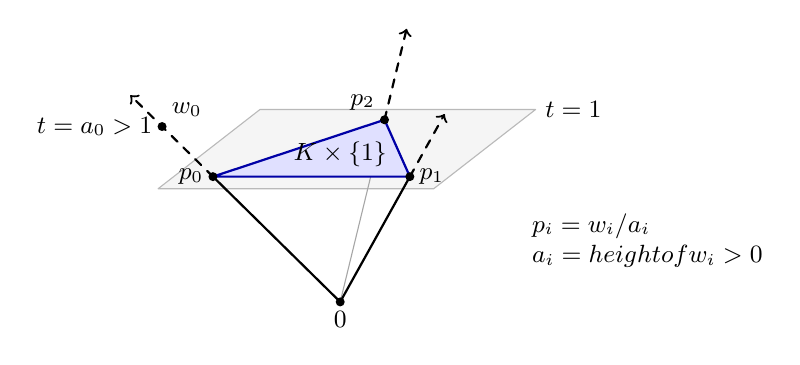
\begin{tikzpicture}[scale=1.25,
    x={(1cm,0cm)},y={(0.45cm,0.35cm)},z={(0cm,1.5cm)},
    line cap=round,line join=round,font=\small]
  \coordinate (O) at (0,0,0);
  \coordinate (P0) at (-1,-0.65,1);
  \coordinate (P1) at (1,-0.65,1);
  \coordinate (P2) at (0,1,1);
  \coordinate (W0) at (-1.4,-0.91,1.4);
  \fill[gray!8] (-1.4,-1,1)--(1.4,-1,1)--(1.4,1.3,1)
    --(-1.4,1.3,1)--cycle;
  \draw[gray!55] (-1.4,-1,1)--(1.4,-1,1)--(1.4,1.3,1)
    --(-1.4,1.3,1)--cycle;
  \node[anchor=west] at (1.4,1.3,1) {$t=1$};
  \draw[gray!70] (O)--(P2);
  \fill[blue!12] (P0)--(P1)--(P2)--cycle;
  \draw[blue!65!black,thick] (P0)--(P1)--(P2)--cycle;
  \draw[thick] (O)--(P0) (O)--(P1);
  \draw[thick,dashed,->] (P0)--(-1.65,-1.0725,1.65);
  \draw[thick,dashed,->] (P1)--(1.5,-0.975,1.5);
  \draw[thick,dashed,->] (P2)--(0,1.5,1.5);
  \fill (W0) circle[radius=1.3pt]
    node[above right] {$w_0$} node[left] {$t=a_0>1$};
  \fill (O) circle[radius=1.3pt] node[below] {$0$};
  \fill (P0) circle[radius=1.3pt] node[left] {$p_0$};
  \fill (P1) circle[radius=1.3pt] node[right] {$p_1$};
  \fill (P2) circle[radius=1.3pt] node[above left] {$p_2$};
  \node at (0,0,1) {$K\times\{1\}$};
  \node[align=left,anchor=west] at (2.3,-1,0.65)
    {$p_i=w_i/a_i$\\$a_i=\text{height of }w_i>0$};
\end{tikzpicture}
\caption{The height-one section of a cone generated by three independent
rays.  Dividing each generator $w_i$ by its positive height $a_i$
produces the vertices $p_i$ of the section; one generator above the
section is shown explicitly.  Formula
\eqref{eq:body-cone-section} gives the same correspondence in every
dimension.}
\label{fig:cone-section}
\end{figure}
